\section{EAP Method Definition}
We want to encapsulate our extended zero-knowledge authentication system defined in \S\ref{label:protocol-design}  as an EAP method in the EAP framework we've explored in \S\ref{section:eap}.
To achieve this we must define a new EAP method, which consists of messages exchanged between the \textit{peer} and the \textit{authenticator}, their data formats and how processes for handling them.

\paragraph{Terminology}
In this section we will be using EAP terminology as described in \S\ref{section:eap}, which uses different names to describe parties involved, as the ones used in our system architecture in \S\ref{label:protocol-design} or as in the ZKP protocol in \S\ref{zkp-qrp}.
The two parties in EAP are called the peer and the authenticator, where the peer is authenticating with the authenticator.
To draw parallels between our system architecture, where we use the names \textit{user} and \textit{authentication system}, the peer is the user and the authenticator is the authentication system.
In the ZKP protocol names \textit{prover} and \textit{verifier} are used, the peer is the prover, and the authenticator is the verifier.


%\subsection{Method Definition}

\bigskip
\noindent
To define an EAP method we need to break down our authentication system described in \S\ref{label:protocol-design} to EAP messages representing interactions between the user and the authentication system.
Each message defines its data format, the sender and recipient processes and local state changes.
Our EAP method defines of two message pairs, the \textit{setup} message pair and the \textit{verification} message pair.
The message pairs are not an identical mapping to the exchanges as described in \S\ref{zkp-qrp}, but are slightly interlaced to optimise the number of messages sent for a successful authentication.

Our authentication system was designed for systems with multiple users, for this reason the authenticator needs to start the authentication process by querying the identity of the peer with the \textit{identity} (type 1) EAP message.
The \textit{setup} message pair is used for discovery of ZKP parameters by the peer, and to provide the values for the first proof verification round to the authenticator.
This message pair is exchange only once.
The \textit{verification} message pair is used to exchange data required for a single round of proof verification. Since proof verification as described in \S\ref{zkp-qrp} requires $m$ iterations, this message pair is exchange $m$ times.
The protocol ends with the authenticator sending either a \textit{success} or a \textit{failure} message.

%TODO: Change title
\subsubsection{Authentication steps}
Let us examine the steps involved in authentication with our EAP method. We are going to be referencing messages displayed in the sequence diagram in \ref{fig:eap-84}.
The purpose of this section is to visually aid the understanding of the authentication process, meaning that some nuances are left our for the purpose of simplification, a detailed definition of individual messages is in the next section.

The mathematical variables have the same meaning as in the system architecture described in \S\ref{label:protocol-design}, this applies to all further sections.

\begin{figure}[h!]
	\centering
	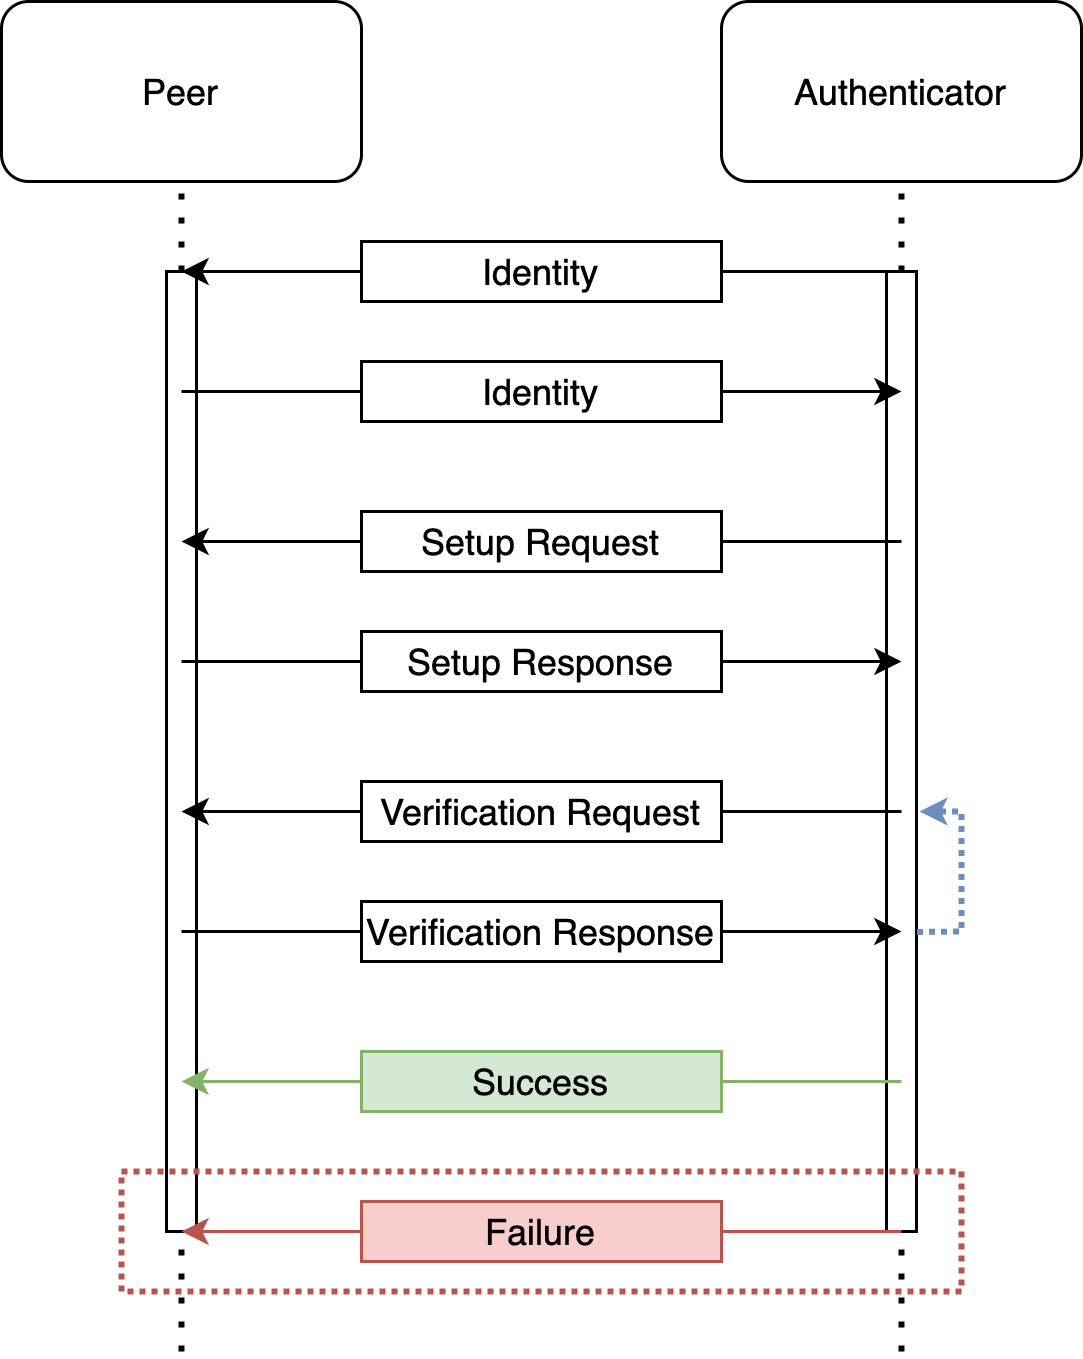
\includegraphics[width=10cm]{images/eap-zkp}
	\caption{EAP Method Execution}
	\label{fig:eap-84}
\end{figure}

\newpage
\begin{description}
	\item [Identity] This message is used to query the identity of the peer. In a system with multiple users this is required to identify the peer authenticating, but more specifically the authenticator needs to find the correct salt $s$ and quadratic residue $x$. 
	\item [Setup] The peer needs both the salt $s$ and the modulus $n$ to compute the proof, however he only know the password $p$. Once the peer identifies himself, the authenticator needs to send him the salt $s$ and modulus $n$ in the \textit{setup request} message.
	\item [Verification] With this message pair the peer and the authenticator exchange data to compute and verify the ZKP. The authenticator send the random bit $b$ and the peer responds with the proof $z$. The peer also sends the control value $y_{i+1}$ for the next verification round $i+1$, this is done as an optimisation to improve the speed of the process.
	\item [Success/Failure] After each \textit{verification} message, the authenticator verifies the proof, and once it was successfully verified for $m$ rounds, the authenticator sends the \textit{success} message. However at anytime if the proof isn't valid the authenticator must send a \textit{failure} message.
\end{description}

\subsubsection{Method \textit{Type} and \textit{Sub-Type}}
Our EAP method is identified by the \textit{type} number $84$.
The message pairs of the EAP method are identified by the \textit{sub-type} field within the \textit{type data}.
\begin{itemize}
	\item Setup (Sub Type 1)
	\item Verification (Sub Type 2)
\end{itemize}

\subsubsection{Key-Stretching Method}
Our architecture does not specify a key-stretching method, and neither does this EAP method.
We assume that in a practical implementation the method would be pre-defined and implicitly known by both parties, without the need for discovery.

\subsection{Setup Message Pair}
In our architecture we assumed the modulus $n$ and salt $s$ are known by the user, however the EAP method needs to facilitate the discovery of this data.
The response message additionally contains the control value $y_1$, used to verify the proof in the fist verification round. The data is already included in this message to improve the method performance.

We are assuming that in a system with multiple users, the authenticator has identified the peer with the \textit{identity} message.

\subsubsection{Request} Message is used to deliver the salt $s$ and semiprime modulus $n$ to the peer.

\paragraph{Data Format}

\begin{center}
\begin{tabular}{|c|c|c|c|c|}
	\hline
	Length (Octets) & ... & 1 & $4 \le k \le 255 $ & $64 \le j$\\
	\hline
	Field Type & ... & Salt Length & Salt & Modulus\\
	\hline
\end{tabular}
\end{center}

\begin{description}
	\item[Salt Length] A single octet for the length of the \textit salt field in octets.
	\item[Salt] A random salt value, should be from 4 octets to 255 octets long.
The max length is determined by the largest number able to be encoded in the \textit {salt length} field.
	\item[Semiprime Modulus] Fills the rest of the message to the length specified by the \textit{length} field in the EAP message. 
Should be at least 64 octets (512 bits).
\end{description}

\paragraph{Request Handling} When a request is received, the peer computes the secret $w$ using the password $p$ the salt $s$ with the pre-determined hashing function $H$.
$$w = H(p, s)$$
Secret value $w$ should be stored stored in memory by the peer. 
Next the peer should pick a random integer $u$ from field $Z^*_n$, and store it in memory and then compute the control value $y = u^2 \Mod{n}$.
The control value $y$ is included in the response message.

\subsubsection{Response}
The response contains the control value $y_1$ to the authenticator to be used in the first round of the verification process.
The subscript of a variable $y_i$ denotes in which verification round $i$ is the variable used.

\paragraph{Data Format}

\begin{center}
\begin{tabular}{|c|c|c|}
	\hline
	Length (Octets) & ... & $k$ \\
	\hline
	Field Type & ... & Control Value $y_1$\\
	\hline
\end{tabular}
\end{center}

\bigskip

\begin{description}
	\item[Control Value] Computed by the peer, where $y_1 = u_1^2 \Mod{n}$ and $u_1 \leftarrow_R \mathbb{Z}^*_n$.
\end{description}

\paragraph{Response Handler}
The authenticator should store the $y_1$ control value locally to be used when verifying the proof $z_1$.

\subsection{Verification Message Pair}
The purpose of this message pair is to exchange data required to compute and verify the proof.
It is continuously exchanged until the authentication is concluded.
After $m$ successful rounds, when the authenticator reaches a confidence of $1 - 2^{-m}$ in the proof, the authentication is successful.

To make our method more efficient, we reduce the number of exchanged messages between the parties by interlacing some data between iterations.
On the round $i$, the response contains data required for the round $i+1$.


\subsubsection{Request}
In the round $i$, the authenticator generates random bit $b_i$ stores it locally, and sends it to the peer.
\paragraph{Data Format}

\begin{center}
\begin{tabular}{|c|c|c|}
	\hline
	Length (Octets) & ... & $1$ \\
	\hline
	Field Type & ... & Random Bit $b_i$\\
	\hline
\end{tabular}
\end{center}

\begin{description}
	\item[Random Bit] A single-bit $b_i$, at the right-most place. 1 octet long.
\end{description}

\paragraph{Request Handling}
The peer computes the proof $z_i = u_iw^{b_i} \Mod{n}$, with the bit $b_i$ received in the request.

Additionally the peer generates the control value $y_{i+1}$ for the next ($i+1$) verification round.
The peer picks a random integer $u_{i+1}$ from field $Z^*_n$ and stores it in memory.
The control value is computed as $y_{i+1} = u_{i+1}^2 \Mod{n}$ and sent in the response.

\subsubsection{Response}

The response transmits the proof $z_i$ and the control value $y_{i+1}$ to the authenticator, who verifies the proof and makes a decision on how to proceed.
\paragraph{Data Format}

\begin{center}
\begin{tabular}{|c|c|c|c|c|}
	\hline
	Length (Octets) & ... & $1$ & $k $ & $j$\\
	\hline
	Field Type & ... & Proof Length & Proof $z_i$ & Control Value $y_{i+1}$\\ %TODO: Witness, check if this is the correct term?
	\hline
\end{tabular}
\end{center}

\begin{description}
	\item [Proof Length] A field one octet in length. Determines the length of the Proof field in octets.
	\item [Proof] Value $z_i$ computed by the peer, verified by the authenticator.
	\item [Control Value] Value $y_{i+1}$, required to verify the proof of the $(i+1)$-th round.
\end{description}

\paragraph{Response Handling}
The authenticator should verify the proof by asserting that $z_i^2 \equiv y_ix^{b_i} \Mod{n}$.
If the verification fails the a \textit{failure} message must be sent to the peer, otherwise a \textit{success} message must be sent if the verification was successful for $m$ rounds.
If that is not the case, the $y_{i+1}$ is stored by the authenticator and a new verification message request is sent.

%\subsection{Optimisations}
%EAP is a lock-step protocol, the authenticator and the peer exchange request and response messages.
%
%A naive mapping of PBA-ZKP-QRP messages to EAP packets yields 3 new request/response pairs. 
%We can reduce the amount of new pairs to 2 instead of 3, by interlacing data shared in each pair.
%This way we obtain a faster performance by reducing the number of packet needed to be exchanged.
%
%\subsubsection{Naive Map}
%
%\begin{center}
%	\begin{tabular}{c|rcl}
%	Pair & Peer  & $\leftrightarrow$ & Authenticator \\
%	\hline
%	1 & & $\xleftarrow{s, n}$ &\\
%	&& $\xrightarrow{\textvisiblespace}$&\\
%	\hline
%	2 & & $\xleftarrow{\textvisiblespace}$&\\
%	&& $\xrightarrow{y}$&\\
%	\hline
%	3 & & $\xleftarrow{b}$&\\
%	&& $\xrightarrow{z}$&\\
%	\hline
%	\end{tabular}
%\end{center}
%
%\paragraph{Pair 1} Exchanged once after the authenticator obtaining the peers identity. The authenticator sends the salt $s$ and semiprime modulus $n$ to the peer, in order for the peer to compute the private input $w$. 
%Peers response serves as an acknowledgement of a successful setup.
%
%This pair corresponds to the \textit{setup} part of the protocol.
%
%\paragraph{Pair 2} The authenticator requests the peer to generate the \textit{square} value $y$ and share it in the response.
%
%This pair corresponds to the ZKP-QRP part of the protocol and is repeated for $m$ times. %TODO: Update the terminology to use ZKP-QRP everwhere
%
%\paragraph{Pair 3} The authenticator requests the peer to compute the \textit{witness} value $z$, with the value of the random bit $b$ in the request data.
%
%This pair corresponds to the ZKP-QRP part of the protocol and is repeated for $m$ times.
%
%\paragraph{Performance}
%With this mapping a successful protocol run of $m$ iterations with a probability of error of $2^{-m}$, would require a minimum of $4m + 3$ packet exchanges.
%
%\bigskip
%
%\begin{center}
%	\begin{tabular}{r|l}
%		Packets exchanged & Type\\
%		\hline
%		2 & Pair 1\\
%		$2m$ & Pair 2\\
%		$2m$ & Pair 3\\
%		1 & Type 2 (Success)\\
%	\end{tabular}
%\end{center}
%
%\subsubsection{Interlaced Data Mapping}
%
%\begin{center}
%	\begin{tabular}{c|rcl}
%	Pair & Peer  & $\leftrightarrow$ & Authenticator \\
%	\hline
%	1 & & $\xleftarrow{\text{s, n}}$ &\\
%	&& $\xrightarrow{y_1}$&\\
%	\hline
%	2 & & $\xleftarrow{b}$&\\
%	&& $\xrightarrow{z, y_{n+1}}$&\\
%	\hline
%	\end{tabular}
%\end{center}
%
%\paragraph{Pair 1} Exchanged once after the authenticator obtains the peers identity. 
%The authenticator sends the salt $s$ and semiprime modulus $n$ to the peer, in order for the peer to compute the private input $w$.
%Peer computes the square value $y$ and sends it in the response.
%
%The main difference with the naive mapping is that the peer responds prematurely with $y$, instead of in the response to naive pair 2. %TODO: Reword, weird sentence
%This is possible and valid, because the semiprime modulus value $n$ required to compute $y$, is provided in the pair 1 request.
%
%\paragraph{Pair 2}
%The authenticator already has the square value $y$, and sends a request with a random bit $b$. 
%The peer computes sends the \textit{witness} $z$ and the square value $y_{n+1}$, used in the next iteration of the protocol
%
%This is possible because the computation of square value $y$ is only dependent on the modulus $n$, which is provided in the request pair 1.
%
%\paragraph{Performance}
%With this mapping a successful protocol run of $m$ rounds with an error rate $2^{-m}$, would require a minimum of $2m + 3$ packet exchanges.
%
%\begin{center}
%\begin{tabular}{r|l}
%	Packets exchanged & Type\\
%	\hline
%	2 & Pair 1\\
%	$2m$ & Pair 2\\
%	1 & Type 2 (Success)\\
%\end{tabular}
%\end{center}
%
%Comparing the performance of both mappings, the interlaced mapping requires half as many exchanges for the same $m$ rounds of protocol.
%
%$$\lim_{1 \rightarrow \infty} \frac{2m + 3}{4m + 3} = \frac{1}{2}$$
%
%\bigskip
%\subsection{Security}
%EAP PB-ZKP-QRP is resistant to passive attacks to over-the-wire information, eavesdropping, active attacks and offline attacks with pre-computed tables/rainbow tables.
%
%The protocol does not enable mutual authentication, nor helps in deriving a session key that can be used for data encryption.
